% Options for packages loaded elsewhere
\PassOptionsToPackage{unicode}{hyperref}
\PassOptionsToPackage{hyphens}{url}
%
\documentclass[
]{article}
\usepackage{amsmath,amssymb}
\usepackage{lmodern}
\usepackage{float}
\usepackage{ifxetex,ifluatex}
\usepackage{xcolor}
\usepackage{listings}

\definecolor{lightgrey}{rgb}{0.93,0.93,0.93}
\lstset{basicstyle=\ttfamily\footnotesize,
  showstringspaces=false,
  breaklines=true,
  columns=flexible,
  numbersep=5pt,
  captionpos=b,
  showspaces=false,
  showstringspaces=false,
  commentstyle=\color{red},
  keywordstyle=\color{blue},
  backgroundcolor=\color{lightgrey},
    frame=lines
}

\definecolor{eclipseStrings}{RGB}{42,0.0,255}
\definecolor{eclipseKeywords}{RGB}{127,0,85}
\colorlet{numb}{magenta!60!black}

\lstdefinelanguage{json}{
    basicstyle=\tiny\ttfamily,
    commentstyle=\color{eclipseStrings}, % style of comment
    stringstyle=\color{eclipseKeywords}, % style of strings
    showstringspaces=false,
    showspaces=false,
    breaklines=true,
    frame=lines,
    string=[s]{"}{"},
    comment=[l]{:\ "},
    morecomment=[l]{:"},
    literate=
        *{0}{{{\color{numb}0}}}{1}
         {1}{{{\color{numb}1}}}{1}
         {2}{{{\color{numb}2}}}{1}
         {3}{{{\color{numb}3}}}{1}
         {4}{{{\color{numb}4}}}{1}
         {5}{{{\color{numb}5}}}{1}
         {6}{{{\color{numb}6}}}{1}
         {7}{{{\color{numb}7}}}{1}
         {8}{{{\color{numb}8}}}{1}
         {9}{{{\color{numb}9}}}{1}
}

\definecolor{codegreen}{rgb}{0,0.6,0}
\definecolor{codegray}{rgb}{0.5,0.5,0.5}
\definecolor{codepurple}{rgb}{0.58,0,0.82}
\definecolor{backcolour}{rgb}{0.95,0.95,0.92}

\lstdefinestyle{mystyle}{
    backgroundcolor=\color{backcolour},   
    commentstyle=\color{codegreen},
    keywordstyle=\color{magenta},
    numberstyle=\tiny\color{codegray},
    stringstyle=\color{codepurple},
    basicstyle=\tiny\ttfamily\footnotesize,
    breakatwhitespace=false,         
    breaklines=true,                 
    captionpos=b,                    
    keepspaces=true,                 
    numbers=left,                    
    numbersep=5pt,                  
    showspaces=false,                
    showstringspaces=false,
    showtabs=false,                  
    tabsize=2
}
\ifnum 0\ifxetex 1\fi\ifluatex 1\fi=0 % if pdftex
  \usepackage[T1]{fontenc}
  \usepackage[utf8]{inputenc}
  \usepackage{textcomp} % provide euro and other symbols
\else % if luatex or xetex
  \usepackage{unicode-math}
  \defaultfontfeatures{Scale=MatchLowercase}
  \defaultfontfeatures[\rmfamily]{Ligatures=TeX,Scale=1}
\fi
% Use upquote if available, for straight quotes in verbatim environments
\IfFileExists{upquote.sty}{\usepackage{upquote}}{}
\IfFileExists{microtype.sty}{% use microtype if available
  \usepackage[]{microtype}
  \UseMicrotypeSet[protrusion]{basicmath} % disable protrusion for tt fonts
}{}
\makeatletter
\@ifundefined{KOMAClassName}{% if non-KOMA class
  \IfFileExists{parskip.sty}{%
    \usepackage{parskip}
  }{% else
    \setlength{\parindent}{0pt}
    \setlength{\parskip}{6pt plus 2pt minus 1pt}}
}{% if KOMA class
  \KOMAoptions{parskip=half}}
\makeatother
\usepackage{xcolor}
\IfFileExists{xurl.sty}{\usepackage{xurl}}{} % add URL line breaks if available
\IfFileExists{bookmark.sty}{\usepackage{bookmark}}{\usepackage{hyperref}}
\hypersetup{
  hidelinks,
  pdfcreator={LaTeX via pandoc}}
\urlstyle{same} % disable monospaced font for URLs
\usepackage{color}
\usepackage{fancyvrb}
\usepackage{graphicx}
\makeatletter
\def\maxwidth{\ifdim\Gin@nat@width>\linewidth\linewidth\else\Gin@nat@width\fi}
\def\maxheight{\ifdim\Gin@nat@height>\textheight\textheight\else\Gin@nat@height\fi}
\makeatother
% Scale images if necessary, so that they will not overflow the page
% margins by default, and it is still possible to overwrite the defaults
% using explicit options in \includegraphics[width, height, ...]{}
\setkeys{Gin}{width=\maxwidth,height=\maxheight,keepaspectratio}
% Set default figure placement to htbp
\makeatletter
\def\fps@figure{htbp}
\makeatother
\setlength{\emergencystretch}{3em} % prevent overfull lines
\providecommand{\tightlist}{%
  \setlength{\itemsep}{0pt}\setlength{\parskip}{0pt}}
\setcounter{secnumdepth}{-\maxdimen} % remove section numbering
\ifluatex
  \usepackage{selnolig}  % disable illegal ligatures
\fi

\begin{document}
\begin{titlepage}
     {
\includegraphics[width=0.4\textwidth]{dssic.png}\par}
\vspace{1cm}
      \vspace{3cm}
    {\scshape\Huge\noindent Trabajo final ICP\\\centering  Serverless Computing\par}
         \vspace{2cm}
{\Large Manuel José Martínez Baños\par}
\vfill
{\Large Febrero de 2021 \par}
  \centering
 \end{titlepage}
%%%%%%%%%%%%%%%%%%%%%%%%%%%%%%%%%%%%%%%%%%%%%%%%%%%%%%%%%%%%%%%%%%%%

%%%%%%%%%%%%%%%%%%%%%%%%%%%%%%%%%%%%%%%%%%%%%%%%%%%%%%%%%%%%%%%%%%%%
% Indice %
%%%%%%%%%%%%%%%%%%%%%%%%%%%%%%%%%%%%%%%%%%%%%%%%%%%%%%%%%%%%%%%%%%%%
\tableofcontents 
\cleardoublepage %terminar la pagina en blanco, salto de pagina


\hypertarget{header-n2}{%
\section{Abstract}\label{header-n2}}

Hoy en día el termino \emph{cloud computing} no forma parte de un futuro
cercano, es ya una realidad que hace tiempo llego a un estado de
madurez. A raíz de ello, han empezado a coger fuerza otras tendencias
tecnológicas como el caso de \emph{serverless
computing}\protect\hyperlink{1}{{[}5{]}}.

Hay que aclarar que el nombre \emph{serverless computing} puede llevar a
confusión, no significa computación sin necesidad de servidor, la parte
"\emph{less}" de serverless significa brindar a los
clientes de no tener que administrar el servidor que ejecutas sus
aplicaciones. En este paradigma, se factura las tareas en función del
uso real de recursos que precisa cada aplicación o tarea en específico.
A grandes rasgos y enfocándose en su uso más básico, \emph{serverless
computing} proporciona la ventaja de simplificar el proceso de
implementación de código en un escenario de producción. Por tanto, se
abaratan los costes y se agiliza la implementación, siendo proveedor
cloud el encargado de las tareas como el escalado de recursos en función
de la demanda.

Actualmente, proveedores como Amazon Web Services, Microsoft
Azure\protect\hyperlink{1}{{[}1{]}}, Google
cloud\protect\hyperlink{1}{{[}2{]}} o IBM Cloud
Functions\protect\hyperlink{1}{{[}3{]}} ofrecen ese tipo de tecnología
denominada \emph{functions as service}(Faas). En este trabajo se va a
trabajar sobre la plataforma Amazon Web Services y su servicio AWS
Lambda.

En este documento se muestra el desarrollo de funciones AWS Lambda
seguido de una visión global de las distintas funciones, junto a la
representación gráfica tanto de la arquitectura basada en AWS Lambda
como sus interacciones.

A continuación, son expuestas detalladamente cada una de las funciones
implementadas, prosiguiendo a posteriori con los resultados obtenidos y
posibles mejoras futuras u otras funcionalidades
que se podrían desarrollar a consecuencia de la implementación general
anteriormente mostrada. Para finalmente concluir con unas conclusiones
obtenidas a lo largo de este trabajo.
\newpage
\hypertarget{header-n9}{%
\section{Objetivos}\label{header-n9}}

Existen diferentes aspectos a tener en cuenta cuando tenemos que
trasladar nuestro código para que aproveche realmente las
funcionalidades que AWS lambda ofrece. Es por ello, entender y
comprender como funciona AWS para en un futuro ante un problema o
necesidad poder contar con dicha herramienta.

Por tanto, el objetivo principal de este trabajo es entender y aprender
a utilizar AWS Lambda de un modo más minucioso, junto a los servicios
implicados para ser llevado a cabo. AWS Lambda es de coste reducido, es
por ello, que es importante sacarle el máximo partido y para ello,
existen otros servicios que logran proporcionar mayores ventajas a esta
tecnología.

Para llevar a cabo este objetivo principal, se crean tres funciones
lambda que ejecuta una determinada tarea. En este caso particular, una
función es invocada ante la subida de un fichero en un bucket de S3 y
guardado el resultado en otro bucket S3, una segunda función es llamada
por la invocación por parte de la primera función lambda y, por último,
la tercera función es invocada ante el evento generado por la primera
función al subir su resultado a un Bucket S3.

\hypertarget{header-n14}{%
\section{Metodología}\label{header-n14}}

Para poder abordar el objetivo principal, han sido desarrolladas 3
funciones lambda con diferentes roles, donde debido al resultado o
invocación por parte de una de las tres funciones, se activan las demás
funciones lambda.

Estas funciones, junto a toda implementación servicio necesario para su
funcionamiento, es creado automáticamente mediante Python utilizando la
librería boto3. Para el desarrollo de las funciones se ha hecho uso de
Python3 junto a boto3\footnote{SDK de Amazon Web Services (AWS) para
  Python, permitiendo en Python crear, configurar y administrar
  servicios de AWS}para dos de ella, siendo la última función lambda
desarrollada con Nodejs junto a aws-sdk.

A lo largo de los apartados siguientes, se profundiza en la
implementación y funcionalidad de dichas funciones, así como todos los
elementos necesarios para su correcto desempeño. Empezando con una
visión global de las distintas funciones, mediante la representación
gráfica tanto de la arquitectura basada en AWS Lambda como sus
interacciones. Una vez tenida una visión global se entra en detalle en
cada función implementada.
\newpage
\hypertarget{header-n19}{%
\section{Desarrollo}\label{header-n19}}

A lo largo de este apartado se expone una visión general de la
implementación, prosiguiendo con una descripción individual cada una de
las funciones desarrolladas y terminando explicando como desplegar
automáticamente cada una de las funciones explicadas.

\begin{figure}[H]
\centering
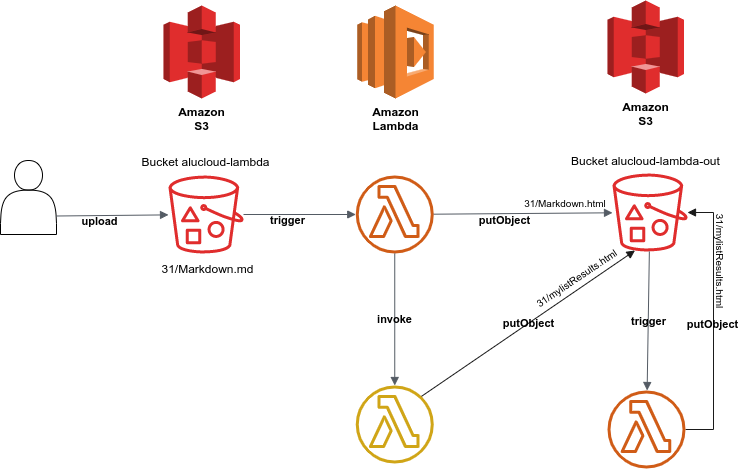
\includegraphics{/home/manu/Documents/MASTER/ICP/Trabajo-Final/Trabajo/docs/diagrams/Deployment_lambda_functions.png}
\caption{Esquema del despliegue resultante}
\end{figure}

Una función lambda se ejecutará cuando se suba un fichero con extensión
\texttt{.md} al bucket de S3 \textbf{alucloud-lambda} en una carpeta (31
para este trabajo) y descargará el fichero del bucket, una vez
descargado lo convertirá a un fichero HTML y posteriormente lo subirá
\textbf{alucloud-lambda-out}. Finalmente invocará a otra función para
que actualice la lista de resultado de las conversiones o tareas
realizadas, ofreciendo el resultado por medio de una página web estática
actualizada).

A su vez, la subida de un fichero con extensión \texttt{.html} al bucket
\textbf{alucloud-lambda-out} provocará la ejecución de una tercera
función. Esta descargará el fichero HTML y filtrará todo el contenido
para obtener solo el texto, generando como resultado un fichero con
extensión \texttt{.txt} que es subido al \textbf{bucket
alucloud-lambda-out.}
\newpage
\hypertarget{header-n24}{%
\subsection{\texorpdfstring{Funciones lambda
}{Funciones lambda }}\label{header-n24}}
Antes de proceder con cada función es necesario poner en contexto sobre
el modelo que se sigue en la programación de las funciones lambda
expuestas anteriormente y detalladas posteriormente. Es necesario
recalcar los aspectos más relevantes que las tres funciones lambda
comparten:

\begin{itemize}
\item
  \textbf{Handler}: Función del código suministrado que el servicio AWS
  Lambda ejecuta cuando la función es invocada. El evento se pasa como
  primer parámetro y como segundo parámetro el \emph{context}.
\item
  \textbf{Context}: Segundo parámetro de la función lambda, utilizada,
  por ejemplo, obtener información que AWS lambda facilita (tiempo
  restante antes que la función termines) o marcar la finalización de
  una función asíncrona mediante ``\emph{context.succeed(`Mensaje de
  finalización')}'' (Utilizada en lenguajes como Nodejs).
\item
  \textbf{Logging}: Todo el mensaje mostrado por salida estándar ( e.g
  \emph{print, console.log, system.out.print}) serán trasladados a
  CloudWatch Logs\footnote{Servicio CloudWatch Logs para monitorizar y
    almacenar archivos de registro, así como obtener acceso a ellos},
  permitiendo ser consultados.
\item
  \textbf{Stateless}: No se asume que el sistema archivos será
  compartido entre las distintas invocaciones de la función lambda. Solo
  /tmp tiene permisos de escrituro, el resto es solo de lectura para
  todo el sistema de archivos.
\end{itemize}

En este trabajo han sido desarrollados 3 funciones lambda que van a ser
detalladas de una manera generalizada a continuación.

\hypertarget{header-n39}{%
\paragraph{Función lambda maestra}\label{header-n39}}
\leavevmode
\newline
\\
Es denominada maestra puesto que será la encargada de realizar la
primera acción, provocando a posteriores la invocación de las dos
funciones restante, ya sea por llamada o por nuevo evento S3. Esta
función tiene como nombre en AWS lambda como
\textbf{lambda-markdown-alucloud31}.

A continuación, las características del código de la función:

\hypertarget{header-n42}{%
\subparagraph{Características}\label{header-n42}}

\begin{itemize}
\item
  Lenguaje Python 3.6
\item
  Librería markdown convertir el fichero a html
\item
  Librería boto3 para interactuar con los servicios de AWS (como S3).
\end{itemize}

\hypertarget{header-n50}{%
\subparagraph{Funcionalidad}\label{header-n50}}
\leavevmode
\newline
\\
Esta función es invocada cuando un fichero Markdown (.md) es subido al
bucket alucloud-lambda y realiza los siguientes pasos:

\begin{enumerate}
\def\labelenumi{\arabic{enumi}.}
\item
  Descarga el nuevo fichero subido
\item
  Lo convierte a formato HTML
\item
  Lo sube al bucket \emph{alucloud-lambda-out}, generando una página web
  estática (importante especificar \emph{Content-Type=text/html})
\item
  Invoca a la función llamada \textbf{lambda-check-alucloud31} con
  información sobre el evento que invoco a la función, el nuevo fichero
  subido e información sobre la propia función (nombre, mensaje,
  resultado ...)
\item
  Obtiene el mensaje de respuesta de la función lambda invocada
\end{enumerate}

El código de la implementación en el anexo sección A.1

Como resultado se obtiene un fichero html generado sobre un markdown:
\begin{figure}[H]
\centering
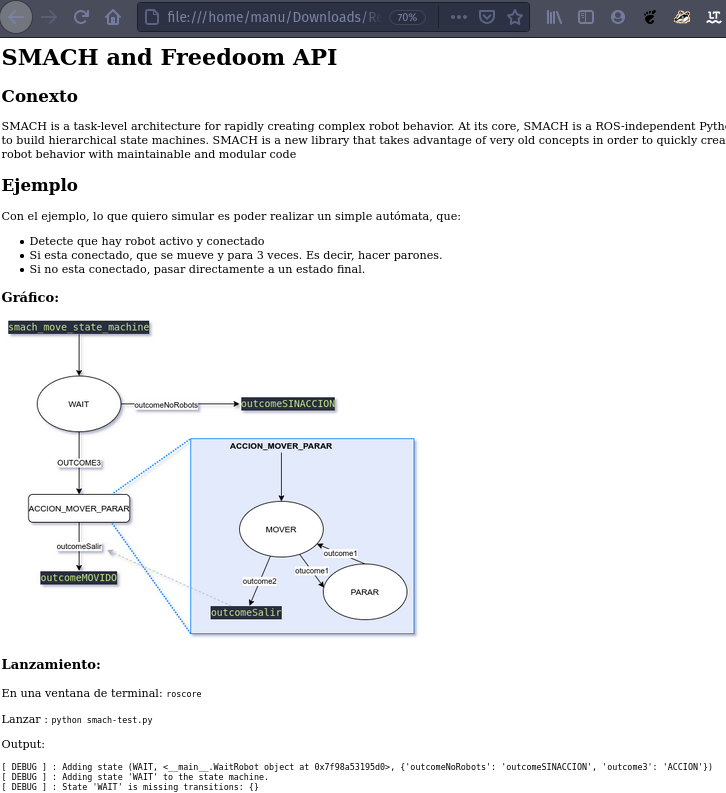
\includegraphics[width=0.6\textwidth]{/home/manu/Documents/MASTER/ICP/Trabajo-Final/Trabajo/docs/imgs/result_html_s3.png}
\caption{Captura de la sección Deploy en AWS Management Console}
\end{figure}

\hypertarget{header-n65}{%
\paragraph{Función lambda hija invocada}\label{header-n65}}
\leavevmode
\newline
\\
Esta función tiene como nombre en AWS lambda como
\textbf{lambda-check-alucloud31}, es invocada por la anterior función
denominada \textbf{lambda-markdown-alucloud31}. Entre estas dos funciones se realiza
la siguiente interacción:
\begin{figure}[H]
\centering
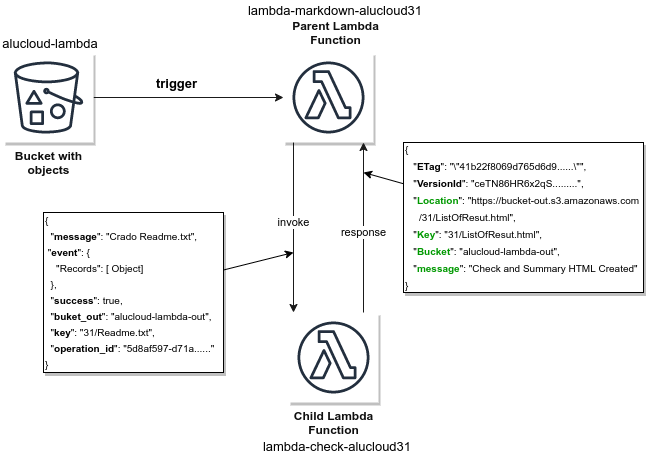
\includegraphics[width=0.9\textwidth]{/home/manu/Documents/MASTER/ICP/Trabajo-Final/Trabajo/docs/diagrams/inter-lambdas-func.png}
\caption{Diagrama de interacción entre lambda-markdown y lambda-check}
\end{figure}
Esta función tiene otras características distintas:

\hypertarget{header-n68}{%
\subparagraph{Características}\label{header-n68}}

\begin{itemize}
\item
  Lenguaje Nodejs12.x
\item
  Librería fs para tratar operaciones de Lectura/Escritura (Permite
  realizar dichas operaciones de forma síncrona)
\item
  Librería aws-sdk para interactuar con los servicios de AWS (como S3).
\end{itemize}

Como podemos observar, entre las características diferenciadoras se
encuentra el lenguaje utilizado. De esta manera, vemos la flexibilidad
que AWS Lambda ofrece y en un futuro permite que este despliegue
mediante funciones lambda no esté ligada a las limitaciones de un solo
lenguaje.

\hypertarget{header-n77}{%
\subparagraph{Funcionalidad}\label{header-n77}}
\leavevmode
\newline
\\
Esta función \textbf{lambda-check-alucloud31} es invocada por la función
\textbf{lambda-markdown-alucloud31} y efectúa los siguientes pasos:

\begin{enumerate}
\def\labelenumi{\arabic{enumi}.}
\item
  Obtiene el mensaje generado por la función invocadora
\item
  Comprueba todas las modificaciones realizadas sobre el bucket
  lambda-bucket-out en una carpeta especificada por el mensaje
  trasmitido
\item
  Realiza un HTML con la información que ha obtenido, generando una
  página web estática.
\item
  Sube el nuevo fichero al bucket alucloud-lambda-out (Especificando el
  tipo de contenido `\emph{text/html}').
\end{enumerate}

El código de la implementación en el \textbf{anexo} sección A.2

Como resultado se obtiene un fichero HTML que actúa como una página web
estática, permitiendo acceder a cada uno de los ficheros creados:

\begin{figure}[H]
\centering
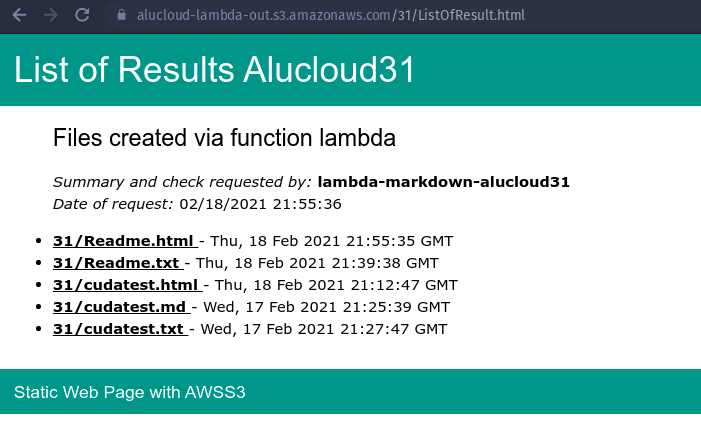
\includegraphics[width=0.8\textwidth]{/home/manu/Documents/MASTER/ICP/Trabajo-Final/Trabajo/docs/imgs/static_web_page_results.png}
\caption{Página web estática generada}
\end{figure}

\hypertarget{header-n92}{%
\paragraph{Función lambda hija}\label{header-n92}}
\leavevmode
\newline
\\
Esta función tiene como nombre en AWS lambda como
\textbf{lambda-html-alucloud31}, función invocada cuando es detectado
como su nombre indica, es la encargada de tratar con ficheros con
extensión \texttt{.html}. A continuación, las características del código
de la función:

\hypertarget{header-n94}{%
\subparagraph{Características}\label{header-n94}}

\begin{itemize}
\item
  Lenguaje Python 3.6
\item
  Librería html2text para convertir el fichero HTML a texto (Además
  filtra todos los patrones de un\\
  HTML)
\item
  Librería boto3 para interactuar con los servicios de AWS (como S3).
\end{itemize}

\hypertarget{header-n102}{%
\subparagraph{Funcionalidad}\label{header-n102}}
\leavevmode
\newline
\\
Esta función \textbf{lambda-html-alucloud31} es invocada cuando un fichero HTML es subido al bucket
alucloud-lambda-out y como\\
consecuencia lleva a cabo los siguientes pasos:

\begin{enumerate}
\def\labelenumi{\arabic{enumi}.}
\item
  Descargar el nuevo fichero subido al bucket \emph{alucloud-lambda-out}
\item
  Realiza su lectura y posterior filtrado del texto.
\item
  El resultado lo sube al mismo bucket de nuevo manteniendo el nombre,
  pero con extensión .txt
\end{enumerate}

El código de la implementación en el anexo sección A.3.
\newline
\hypertarget{header-n112}{%
\subsection{Creación y Lanzamiento}\label{header-n112}}

En el siguiente apartado se muestra y explica cómo se ha llevado a cabo
el despliegue, indicando los elementos o servicios necesarios, paso a
seguir y aspectos a tener en cuenta. Además, se especifica como se ha
llevado a cabo el despliegue automáticamente con ayuda de Python junto a
la librería Boto3. Todo el contenido del trabajo está disponible en el repositorio \underline{\href{https://github.com/manujose94/FINAL-PROJECT-ICP}{FINAL-PROJECT-ICP}}. En ningún momento ha sido subido ninguna información sensible (e.g credenciales, keys, etc.) 

Para realizar el despliegue es necesario tener a disposición:

\begin{itemize}
\item
  Una cuenta de AWS, sus credenciales serán utilizadas para interactuar
  con AWS mediante Boto3
\item
  Los buckets en S3 con los permisos necesarios ( \emph{alucloud-lambda}
  y \emph{alucloud-lambda-cloud} en este caso)
\item
  Un rol con el que se ejecuta la función lambda, aportando los
  privilegios de acceso a las funciones lambda.
\end{itemize}

Partiendo de la base de los puntos anteriores, se procede al despliegue
de las funciones lambda. Los siguientes pasos, cuentan de forma resumida
la configuración seguida, para un detalle más preciso consultar el
código bien comentado del \textbf{anexo} en el apartado B.

Todo ello ha sido realizado con el siguiente orden:

\begin{itemize}
\item
  Se comprueba si la primera función \textbf{lambda-markdown-alucloud31}
  existe, si no existe es creada-
\item
  Ahora se añade una nueva política a la función para que permita ser
  invocado por un ``\emph{trigger}'' del servicio S3 (Se debe
  especificar el \textbf{arn} del bucket alucloud-lambda en cuestión).
\item
  Ahora se agrega el ``\emph{trigger}'' para que sea ejecutado
  automática ante un evento ``\emph{PutObject}'' del bucket
  \emph{alucloud-lambda}.
\item
  Se crea el "\emph{trigger}" con el prefijo "31/" y el sufijo
  \texttt{.md}, antes de añadirlo se comprueba que nuestro disparador no
  existe.
\item
  Es turno de añadir la función \textbf{lambda-html-alucloud31} si no
  existe.
\item
  Añade una nueva política, para permitirla invocación mediante un
  "\emph{trigger}" de S3, pero ahora indicado el bucket \emph{alucloud-
  lambda -out}.
\item
  Se crea el "\emph{trigger}" con el prefijo "31/" y sufijo
  \texttt{.html}, especificando el bucket \emph{alucloud-lambda-out}
\item
  Por último, la función \textbf{lambda-check-alucloud31} se crea,
  siguiendo los mismos puntos de la función anterior, pero sin añadir el
  "\emph{trigger}" para eventos de S3 (\emph{putObject}).
\item
  Para finalizar, solo se debe permitir que esta función sea invocada
  por otra función, se añade una nueva política (\emph{add new policy})
  para permitir a esta nueva función ser invocada por la función
  \textbf{lambda-markdown-alucloud31} (se debe especificar el
  \textbf{arn} de la función lambda invocadora)
\end{itemize}
\leavevmode
\newline
\hypertarget{header-n144}{%
\subsubsection{Implementación automática mediante
script}\label{header-n144}}
\leavevmode
\newline
Para llevar el despliegue automático de los puntos anteriores, se ha
generado una serie de scripts en Python utilizando la librería boto 3.
En concreto se han creado dos ficheros Python, siendo una de las
encargadas de proporciona la configuración adecuada y otra las funciones
para realizar cada uno de los pasos. Para visualizar con más precisión
el código implementado, consultar en el apartado Anexos la sección B.

A continuación, en el siguiente diagrama de clases se visualiza la
estructura y metodología utilizada:

\begin{figure}[H]
\centering
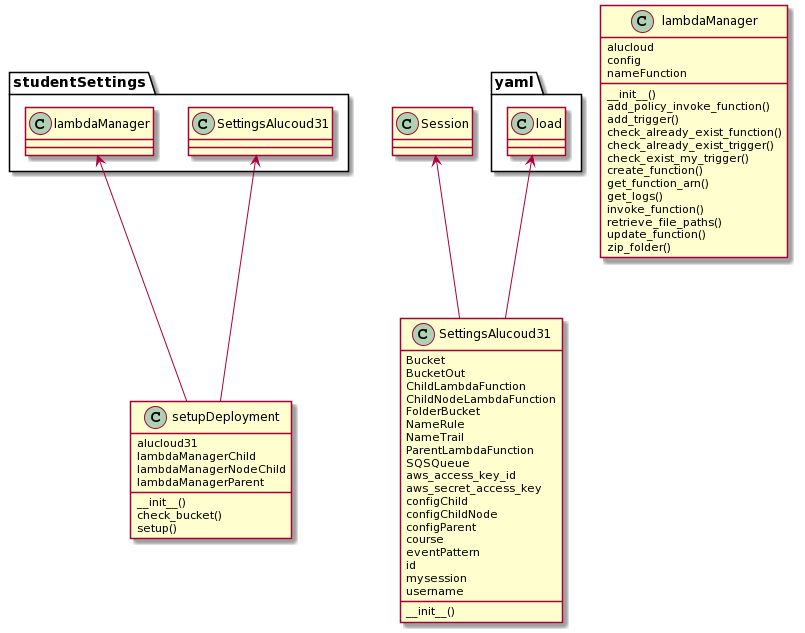
\includegraphics[width=0.9\textwidth]{/home/manu/Documents/MASTER/ICP/Trabajo-Final/Trabajo/docs/imgs/uml_classes.png}
\caption{UML de las clases}
\end{figure}

Como muestra el diagrama existen tres clases:

\begin{itemize}
\item
  \textbf{setupDeployment} creada en el fichero
  \texttt{init-deployment.py} (Anexo B.1)
\item
  \textbf{SettingsAlucloud31} localizada en el fichero
  \texttt{studentSettings.py} (Anexo B.2)
\item
  \textbf{LambdaManager} localizada en el fichero
  \texttt{studentSettings.py} (Anexo B.2)
\end{itemize}
\leavevmode
\newline
\\
\textbf{SettingsAlucloud31}, contiene la configuración con todos los
nombres de los servicios o elementos implicados, así como la sesión de
nuestra cuenta de AWS y la configuración de cada función lambda en
formato YAML.

A continuación, se muestra las 3 configuraciones existentes en la case
SettingsAlucloud31.

\begin{lstlisting}[language=Python, caption=Configuraciones de la clase SettingsAlucloud31]
self.configParent=yaml.load("""
            role: lambda-s3-execution-role
            name: lambda-markdown-alucloud31
            zip: lambda-markdown-alucloud31.zip
            path: parent-lambda-code
            handler: MarkdownConverter.handler
            runtime: python3.6
            description: Convert mardownk documents to html
            suffix: .md
            statementid: '1-lambda'
            bucket: {}
            arn_bucket: arn:aws:s3:::alucloud-lambda
            """.format(self.Bucket), 
            Loader=yaml.FullLoader)
        self.configChild=yaml.load("""
            role: lambda-s3-execution-role
            name: lambda-html-alucloud31
            zip: lambda-html-alucloud31.zip
            path: child-lambda-code
            handler: HTMLConverter.handler
            runtime: python3.6
            description: Just gets the text from the html and generates a txt file
            suffix: .html
            statementid: '2-lambda'
            bucket: {}
            arn_bucket: arn:aws:s3:::alucloud-lambda-out
            """.format(self.BucketOut), 
            Loader=yaml.FullLoader)

        self.configChildNode=yaml.load("""
            role: lambda-s3-execution-role
            name: lambda-check-alucloud31
            zip: lambda-check-alucloud31.zip
            path: childnode-lambda-code
            handler: CheckMyResults.handler
            runtime: nodejs12.x
            description: Invoke by Parent and list his work results.
            suffix: .html,.txt
            statementid: '22-lambda'
            bucket: {}
            arn_bucket: arn:aws:s3:::alucloud-lambda-out
            """.format(self.BucketOut), 
            Loader=yaml.FullLoader)
\end{lstlisting}

Además, por seguridad, las claves nunca son mostradas, son leídas del
fichero \texttt{.env} con el siguiente formato:

\begin{lstlisting}[language=bash,caption={Contenido de .env}]
	ID=<<ID>>
	PREFIXSQS=sqs-alucloud
	PREFIXRULE=alucloud-events-rule-s3-to-sqs-
	USERNAME_AWS=<<NAME_USER>
	KEY_ID=<<HERE KEY>>
	ACCES_KEY=<<HERE ACCES_KEY>>
	REGION=us-east-1
\end{lstlisting}

Nunca será subido al repositorio Git, este \texttt{.env} este añadido al
fichero \texttt{.gitignore} para que en caso de realizar un
``\emph{push}'', no sea subido al repositorio.

\textbf{LambdaManager}, encargada de proporcionar una serie de
funcionalidades para realizar el despliegue. Se instancia, pasándole
como parámetro la instancia de la clase anterior
(\emph{SettingsAlucloud31}), junto a la configuración lambda que
deseamos. A continuación un fragmente de código para ejemplificar:

\begin{lstlisting}[language=Python,caption={Instancias de LambdaManager}]
class setupDeployment:
    def __init__(self):
        self.alucloud31=studentSettings.SettingsAlucoud31()
        self.lambdaManagerParent=studentSettings.lambdaManager(self.alucloud31,self.alucloud31.configParent)
        #Child is invoked when Parent putObject type .html tu Bucket S3
        self.lambdaManagerChild=studentSettings.lambdaManager(self.alucloud31,self.alucloud31.configChild)
        #Node Child is invoked by parent when he finish the task
        self.lambdaManagerNodeChild=studentSettings.lambdaManager(self.alucloud31,self.alucloud31.configChildNode)
\end{lstlisting}

Por cada función se instancia una nueva clase \textbf{LambdaManager}
permitiendo facilitar la gestión individual de cada función.

\textbf{setupDeployment}, es la clase encargada de iniciar el despliegue
utilizando la clase \emph{LambdaManager}para tratar cada función y
\emph{SettingsAlucloud31} para establecer la configuración deseada. A
continuación se muestra como ejemplo, como lanzar o inicializar el
despliegue:

\begin{lstlisting}[language=bash,caption={Iniciar despliegue}]
$ init-deployment.py --Init
\end{lstlisting}

Si ha tenido exito la inicialzación, es motrado la siguigente salida.


\begin{lstlisting}[language=bash,caption={Salida Exitosa}]
[SUCCES] QUEUE sqs-alucloud31 exist
[SUCCES] RULE alucloud-events-rule-s3-to-sqs-31 exist
[SUCCES] FOLDER (31/) on BUCKET (alucloud-lambda)
[SUCCES] FUNCTION LAMBDA(lambda-markdown-alucloud31) exist
[SUCCES] TRIGGER ON BUCKET(alucloud-lambda) exist
[INFO] CHECK OUR TRIGGER ON BUCKET(alucloud-lambda-out) exist
[SUCCES] TRIGGER ON BUCKET(alucloud-lambda) exist
[SUCCES] FUNCTION LAMBDA(lambda-html-alucloud31) exist
[INFO] TRIGGER ON BUCKET(alucloud-lambda-out) exist
[INFO] CHECK OUR TRIGGER ON BUCKET(alucloud-lambda-out) exist
[SUCCES] TRIGGER ON BUCKET(alucloud-lambda) exist
[SUCCES] FUNCTION LAMBDA(lambda-html-alucloud31) exist
\end{lstlisting}

En esta salida, muestra como cada uno de los elementos necesarios para
el despliegue (figura 1) ha sido implementada con éxito.

Además, existen otros parámetros para en un futuro poder ser mejorado,
por ejemplo, esta implementado la visualización de los registros
generados por cada una de las funciones en las últimas 24 horas. Para
obtener los parámetros disponibles:

\begin{lstlisting}{bash,caption=Opción help}
$ init-deployment.py -h

usage: init-deployment.py [-h] [-i INIT] [-l]

optional arguments:
  -h, --help            show this help message and exit
  -i INIT, --Init INIT  Launch the developed setup
  -l, --Logs            Display the logs of each lambda function deployed.
\end{lstlisting}

\hypertarget{header-n172}{%
\subsection{Resultados obtenidos}\label{header-n172}}

A continuación, se muestran imágenes de \textit{AWS Management
Console}\protect\hyperlink{1}{{[}4{]}}, estas son el resultado del
despliegue obtenido:

\textbf{Funciones Lambda desplegadas:}

\begin{figure}[H]
\centering
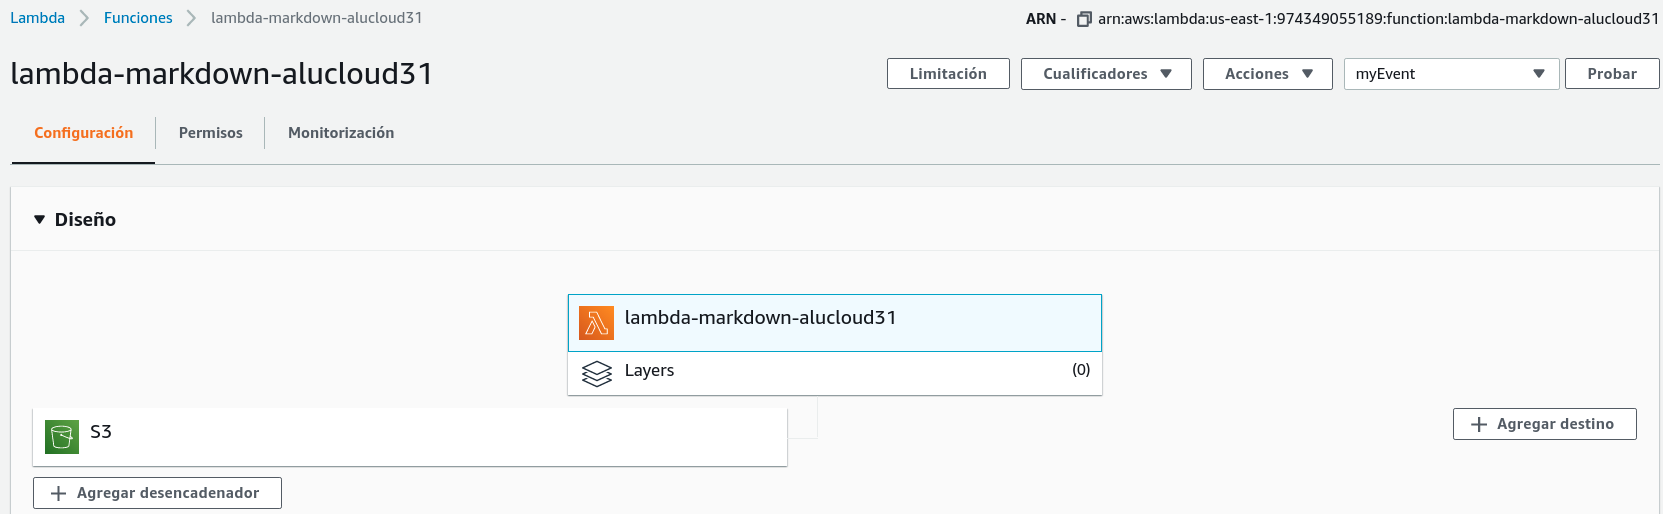
\includegraphics{/home/manu/Documents/MASTER/ICP/Trabajo-Final/Trabajo/docs/imgs/lambda_markdown_with_trigger.png}
\caption{Captura de la función lambda lambda\_markdown\_alucloud31}
\end{figure}

\begin{figure}[H]
\centering
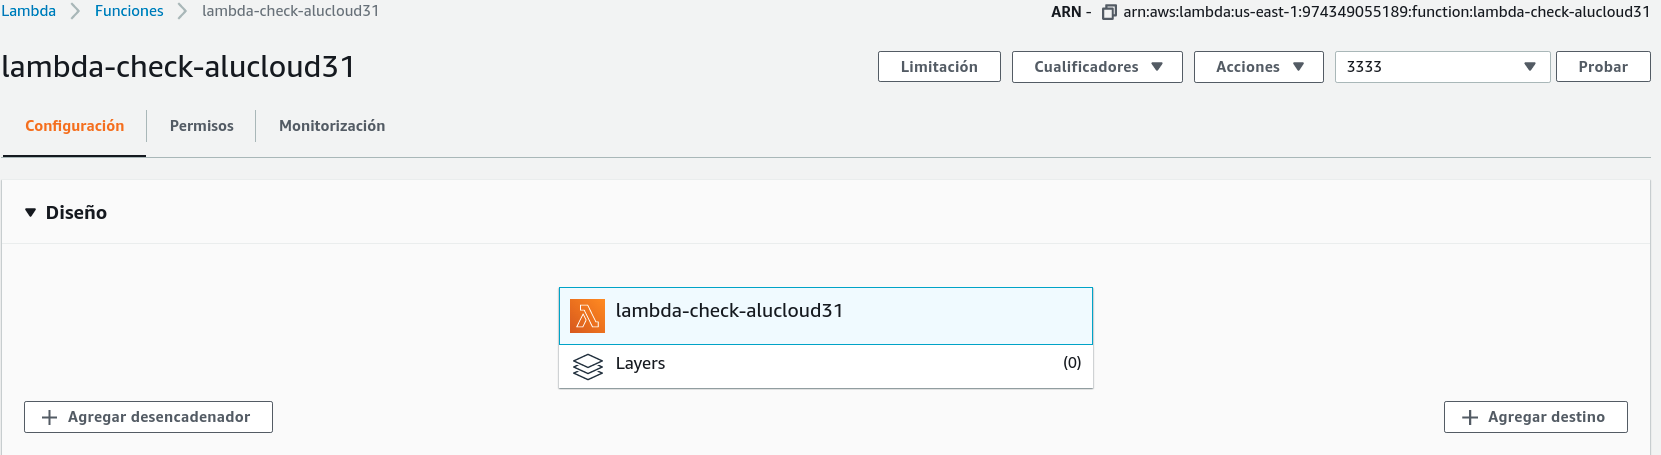
\includegraphics{/home/manu/Documents/MASTER/ICP/Trabajo-Final/Trabajo/docs/imgs/lambda_check_withouth_trigger.png}
\caption{Captura de la función lambda lambda\_check\_alucloud31}
\end{figure}

\begin{figure}[H]
\centering
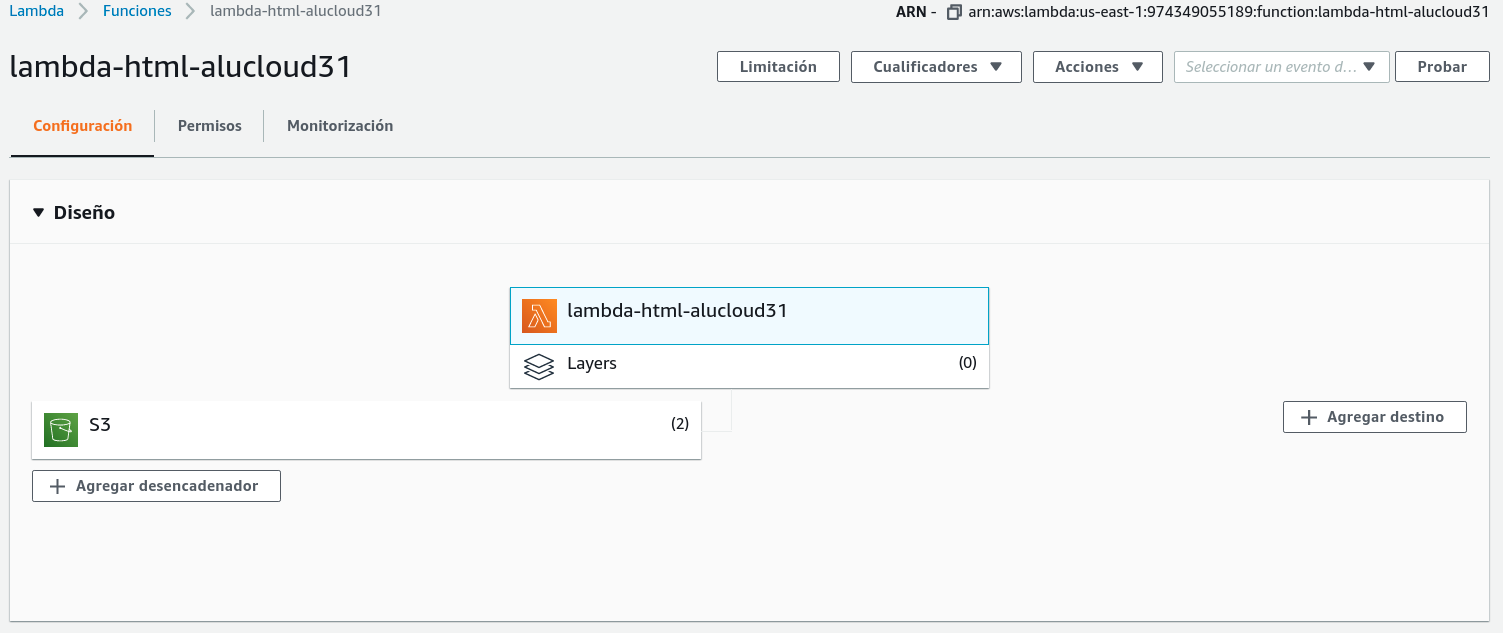
\includegraphics{/home/manu/Documents/MASTER/ICP/Trabajo-Final/Trabajo/docs/imgs/lambda_html_with_trigger.png}
\caption{Captura de la función lambda lambda\_html\_alucloud31}
\end{figure}

\hypertarget{header-n178}{%
\subsection{Pruebas}\label{header-n178}}

En este apartado, se elaboran una serie de pruebas para comprobar el
correcto funcionamiento del despliegue. Para ello, se han realizado una serie de ensayos con el fin de evaluar el despliegue.

\hypertarget{header-n180}{%
\subparagraph{Invocación de la función lambda
lambda-markdown-alucloud31}\label{header-n180}}
\leavevmode
\\
\\
Una de las primeras pruebas es invocar la función lambda-hmtl-alucloud31 mediante la invocación de un evento utilizando una platilla creada previamente (fuente en el Anexo apartado C.1). En este caso, ha sido utilizado la interfaz de líneas de comandos de AWS\footnote{Linea de comandos AWS: https://aws.amazon.com/es/cli/} como medio mayoritario para realizar las pruebas. 
\begin{lstlisting}[language=bash,caption={Comando de invocación mediante plantilla}]
aws lambda invoke \
--invocation-type Event \
--function-name lambda-markdown-alucloud31 \
--region us-east-1 \
--payload file://${PWD}/test_deployment_parent.json \
outputfile.txt
#Successful output: 202
\end{lstlisting}

Registros generados por la invocación:

\begin{lstlisting}[language=bash,caption={Comando para obtener Logs}]
LOG_GROUP=/aws/lambda/lambda-markdown-alucloud31
aws logs get-log-events --log-group-name $LOG_GROUP --log-stream-name `aws logs describe-log-streams --log-group-name $LOG_GROUP --max-items 1 --order-by LastEventTime --descending --query logStreams[].logStreamName --output text | head -n 1` --query events[].message --output text

## Succellfull output
START RequestId: e869dd5f-cc13-437e-b2fd-ca6602e67530 Version: $LATEST
[1] Downloading markdown in bucket alucloud-lambda with key 31/Readme.md
[2] Uploading html in bucket alucloud-lambda-out with key 31/Readme.html
[3] Changing ACLs for public-read for object in bucket alucloud-lambda-out with key 31/Readme.html
[4] Invoke the lambda function lambda-check-alucloud31
Check and Summary HTML Created: File $31/ListOfResult.html with url: https://alucloud-lambda-out.s3.amazonaws.com/31/ListOfResult.html
END RequestId: e869dd5f-cc13-437e-b2fd-ca6602e67530
REPORT RequestId: e869dd5f-cc13-437e-b2fd-ca6602e67530	Duration: 4145.55 ms	Billed Duration: 4146 ms	Memory Size: 128 MB	Max Memory Used: 84 MB	Init Duration: 509.80 ms
\end{lstlisting}

Aquí se muestra como por comandos podemos realizar la invocación de un
evento, utilizado una plantilla de evento creada. Se ha creado una
plantilla distinta para cada evento creado, están disponibles en el
\textbf{anexo} en el apartado C.

Estas plantillas pueden ser lanzadas además, desde \textit{AWS Management
Console}, como se muestra en la siguiente imagen:

\begin{figure}[H]
\centering
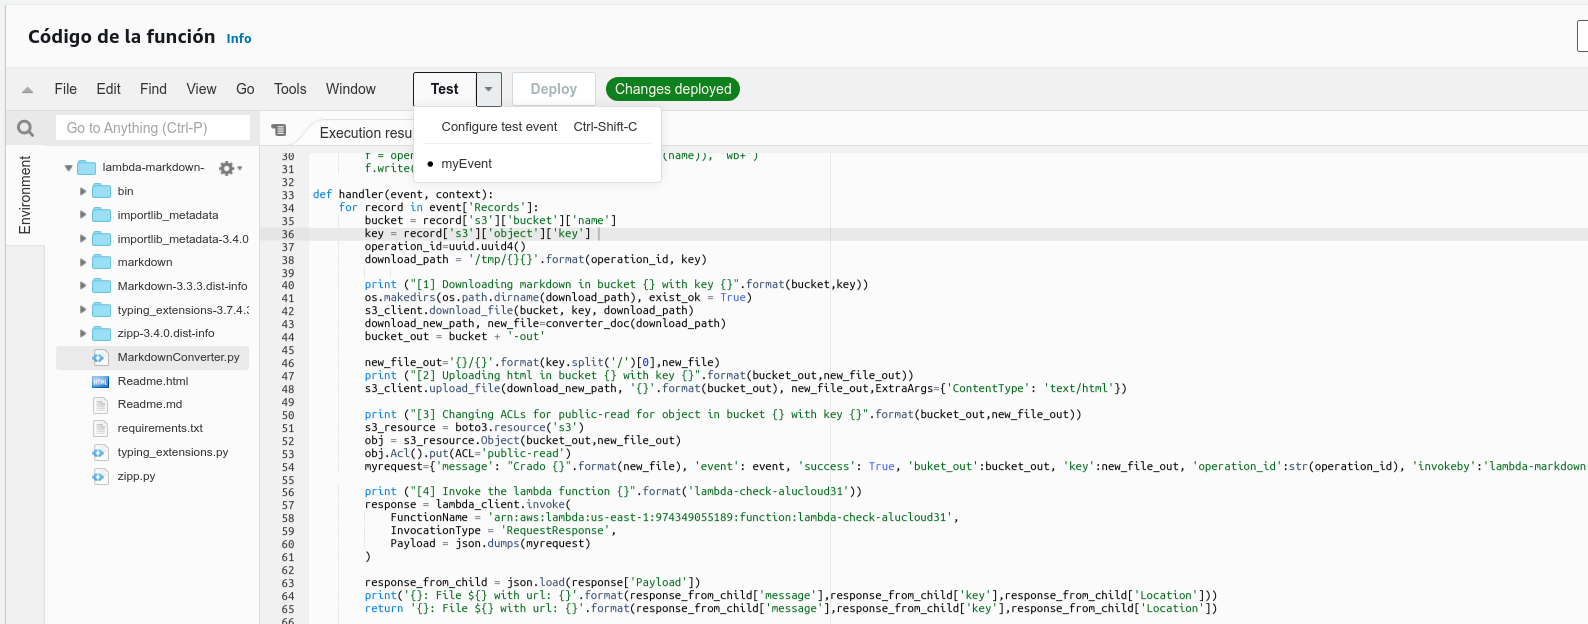
\includegraphics{/home/manu/Documents/MASTER/ICP/Trabajo-Final/Trabajo/docs/imgs/4_functions_lambda_deploy_test.png}
\caption{Captura de la sección Deploy en AWS Management Console}
\end{figure}

Obteniendo como resultado de la ejecución:

\begin{figure}[H]
\centering
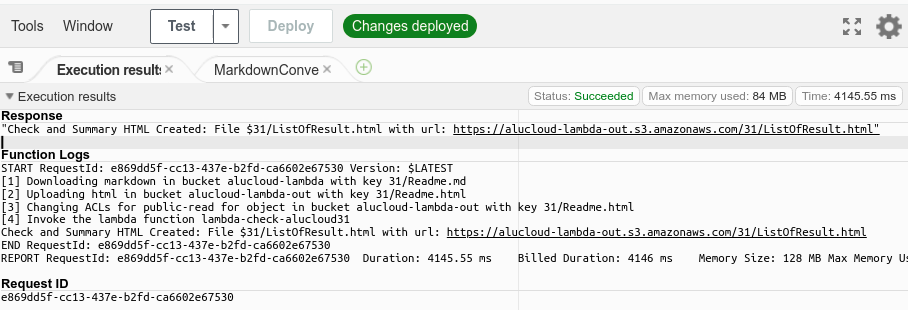
\includegraphics[width=0.9\textwidth]{/home/manu/Documents/MASTER/ICP/Trabajo-Final/Trabajo/docs/imgs/execution_result_markdown.png}
\caption{Captura del resultado al lanzar el Test}
\end{figure}
\hypertarget{header-n190}{%
\subparagraph{Subida de un fichero a S3 y visualización del evento
generado}\label{header-n190}}
\leavevmode
\\
\\
Es posible forzar una subida de un fichero local al bucket deseado, por consiguiente, es comprobado el correcto funcionamiento ante una nueva subida, si todo ha ido correctamente, el resultado final deberá ser un nuevo fichero con formato HTML en el bucket alucloud-lambda-out. 
\begin{lstlisting}[language=bash,caption={Utilizar cp con aws}]
aws s3 cp ${PWD}/example-data/cuda.md s3://alucloud-lambda/$ID/cudatest.md
# Successful output: 
#   upload: example-data/cuda.md to s3://alucloud-lambda-out/31/cudatest.md
\end{lstlisting}

Ahora es listado el fichero en el nuevo bucket:

\begin{lstlisting}[language=bash,caption={Utilizar ls con aws}]
aws s3 ls s3://alucloud-lambda-out/$ID/  | grep --color=always 'cuda'
#Successful output:
#   2021-02-17 21:10:22      13197 cudatest.md
\end{lstlisting}

Por último, esta nueva subida a provocado la la invocación de la función
lambda \textbf{lambda-markdown-alucloud31}, ahora se procede a
visualizar los últimos registros (\emph{logs}) de dicha función.

\begin{lstlisting}[language=bash,caption={Listar logs generados}]
LOG_GROUP=/aws/lambda/lambda-markdown-alucloud31
aws logs get-log-events --log-group-name $LOG_GROUP --log-stream-name `aws logs describe-log-streams --log-group-name $LOG_GROUP --max-items 1 --order-by LastEventTime --descending --query logStreams[].logStreamName --output text | head -n 1` --query events[].message --output text

## Succellfull output
START RequestId: e869dd5f-cc13-437e-b2fd-ca6602e67530 Version: $LATEST
[1] Downloading markdown in bucket alucloud-lambda with key 31/cudatest.md
[2] Uploading html in bucket alucloud-lambda-out with key 31/cudatest.html
[3] Changing ACLs for public-read for object in bucket alucloud-lambda-out with key 31/cudatest.html
[4] Invoke the lambda function lambda-check-alucloud31
Check and Summary HTML Created: File $31/ListOfResult.html with url: https://alucloud-lambda-out.s3.amazonaws.com/31/ListOfResult.html
END RequestId: e869dd5f-cc13-437e-b2fd-ca6602e67530
REPORT RequestId: e869dd5f-cc13-437e-b2fd-ca6602e67530	Duration: 4145.55 ms	Billed Duration: 4146 ms	Memory Size: 128 MB	Max Memory Used: 84 MB	Init Duration: 509.80 ms
\end{lstlisting}

También puede ser visualizado directamente desde \textit{AWS Management Console}
en la siguiente dirección, CloudWatch Logs \textgreater{} Log groups
\textgreater{} /aws/lambda/lambda-markdown-alucloud-31. Aquí se
visualiza la siguiente imagen como ejemplo:

\begin{figure}[H]
\centering
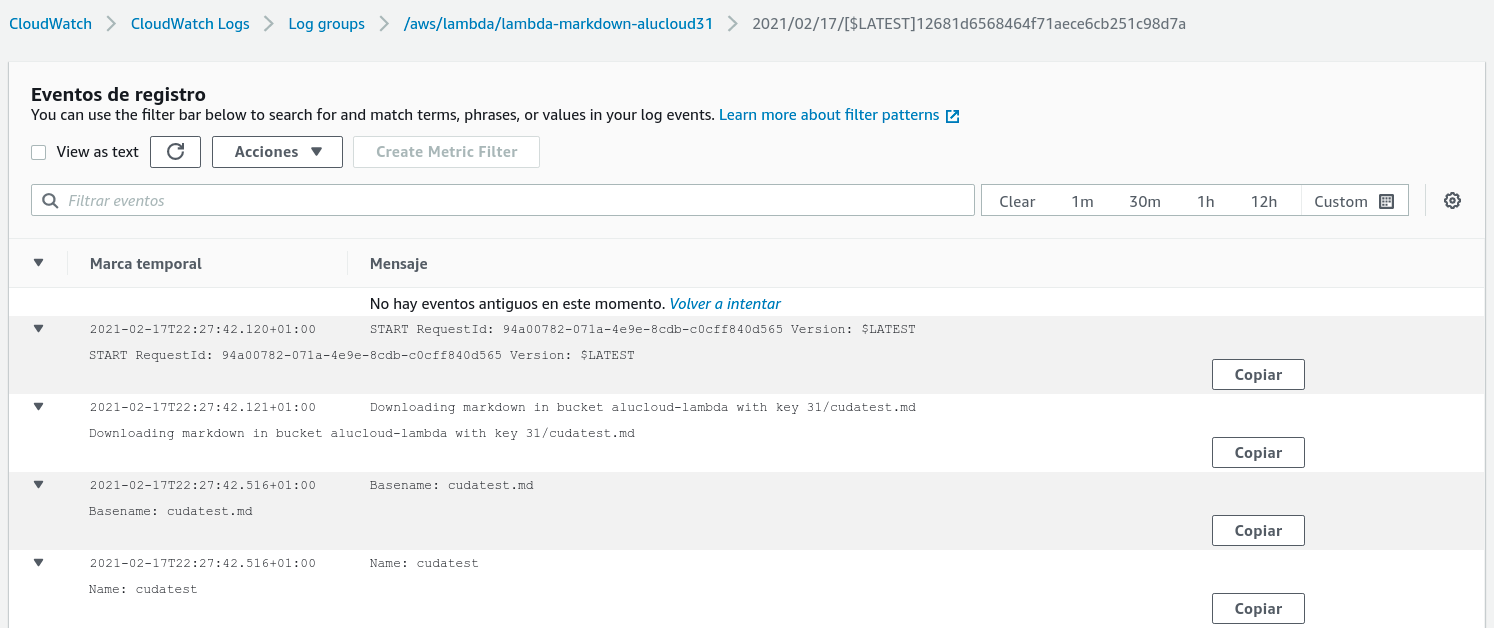
\includegraphics{/home/manu/Documents/MASTER/ICP/Trabajo-Final/Trabajo/docs/imgs/cloudwatch_events_of_lambda_markdown.png}
\caption{Captura de los eventos en CloudWatch Logs}
\end{figure}

Si son observados detalladamente los logs, la función
\textbf{lambda-check-alucloud31} ha funcionado satisfactoriamente, ya
que ha contestado a la invocación de la función testeada. A continuación
la línea que representa la contestación de la función
\textbf{lambda-check-alucloud31} formateada por \textbf{lambda-makdwon-alucloud31} .

\begin{lstlisting}[language=bash,caption={Respuesta}]
Check and Summary HTML Created: File $31/ListOfResult.html with url: https://alucloud-lambda-out.s3.amazonaws.com/31/ListOfResult.html
\end{lstlisting}

Se puede comprobar el mensaje exacto que devuelve la función \textbf{lambda-check-alucloud31}, invocándola y almacenando la respuesta en un fichero. A continuación, un ejemplo: 

\begin{lstlisting}[language=bash,caption={Invocación de la funcion lambda-check-alucloud31}]
# Type of invoke must be RequestResponse
aws lambda invoke --invocation-type RequestResponse --function-name lambda-check-alucloud31 --region us-east-1 --payload file://${PWD}/test_deployment_nodechild.json response.json
$LATEST	200

# Now, showing message content
cat response.json 

{"ETag":"\"a74bd4d61fc0c8b76014e3567c8dc5be\"","VersionId":"i0uwLkpcxhl2zufHMkzNSVK3Sh5SBdc7","Location":"https://alucloud-lambda-out.s3.amazonaws.com/31/ListOfResult.html","key":"31/ListOfResult.html","Key":"31/ListOfResult.html","Bucket":"alucloud-lambda-out","message":"Check and Summary HTML Created"}
\end{lstlisting}

\newpage
\hypertarget{header-n200}{%
\subparagraph{Invocación de la función lambda
lambda-html-alucloud31}\label{header-n200}}
\leavevmode
\\
\\
Probando ahora la función lambda-hmtl-alucloud31 mediante la invocación de un evento utilizando una platilla creada previamente.
\begin{lstlisting}[language=bash,caption={Invocar evento}]
aws lambda invoke \
--invocation-type Event \
--function-name lambda-html-alucloud31 \
--region us-east-1 \
--payload file://${PWD}/test_deployment_child.json \
outputfile.txt
#Successful output: 202
\end{lstlisting}

Una vez a tenido éxito el lanzamiento del evento, es turno de visualizar
los últimos registros de la función.

\begin{lstlisting}[language=bash,caption={Logs de la función}]
LOG_GROUP=/aws/lambda/lambda-html-alucloud31
aws logs get-log-events --log-group-name $LOG_GROUP --log-stream-name `aws logs describe-log-streams --log-group-name $LOG_GROUP --max-items 1 --order-by LastEventTime --descending --query logStreams[].logStreamName --output text | head -n 1` --query events[].message --output text
## Succellfull output
START RequestId: 1029f3e5-3848-44c8-9316-64fa973ca0c2 Version: $LATEST
	[1] Downloading markdown in bucket alucloud-lambda-out with key 31/Readme.html
	[2] Uploading html in bucket alucloud-lambda-out with key 31/Readme.txt
	[3] Changing ACLs for public-read for object in bucket alucloud-lambda-out with key 31/Readme.txt
	END RequestId: 1029f3e5-3848-44c8-9316-64fa973ca0c2
	REPORT RequestId: 1029f3e5-3848-44c8-9316-64fa973ca0c2	Duration: 1462.16 ms	Billed Duration: 1463 ms	Memory Size: 128 MB	Max Memory Used: 78 MB	Init Duration: 477.93 ms	
\end{lstlisting}

Para finalizar las pruebas y confirmar su correcto funcionamiento, se
muestra el resultado con una imágen de la interfaz de \textit{AWS Management
Console}:

\begin{figure}[H]
\centering
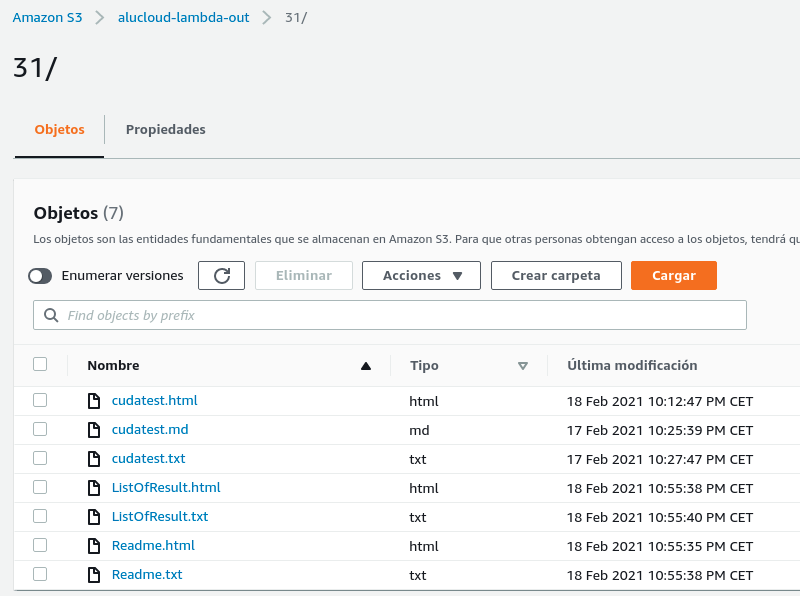
\includegraphics[width=0.8\textwidth]{/home/manu/Documents/MASTER/ICP/Trabajo-Final/Trabajo/docs/imgs/result_s3.png}
\caption{Captura de los resultados generados en el Bucket S3 lambda-alucloud-31}
\end{figure}
\newpage
\hypertarget{header-n206}{%
\section{Futuras Mejoras}\label{header-n206}}

Este apartado tiene como finalidad, plasmar algunas tareas que no han
podido ser realizadas debido al tiempo o aspectos mejorables.

La intención inicial era poder convertir un fichero ".doc" a PDF con
Python, pero debido a que es necesario trabajar con Windows no ha podido
ser posible. Además, las librerías existentes para convertir otros tipos
de documentos a PDF utilizan otras "\emph{sub-librerías}", como
consecuencia a la hora de comprimir el código para ser enviado a AWS,
siempre existe algún error debido a que una librería no es detectada.
Por tanto, para este trabajo se han utilizadas librerías más ligeras
con menos dependencias, permitiendo de ese modo, la posibilidad de
probar y modificar la función desde la propia plataforma de AWS
Management Console.

Para un futuro, es posible tratar cada una de las dependencias o elegir
otro lenguaje, como NodeJs el qual ha sido utilizado.

\hypertarget{header-n210}{%
\section{Conclusiones}\label{header-n210}}
En este trabajo se han mejorado y afianzado los conocimientos previos sobre la arquitectura serverless, obtenidos durante las clases y prácticas de la asignatura de ICP. Además, no solo se ha trabajado con funciones lambda también, con servicios como S3, CloudWatch y visto a groso modo el servicio CloudTrial para el registro de llamadas. 

Como resultado del trabajo realizado se remarca el potencial del servicio AWS Lambda, así como sus ventajas. Ahora no se empieza con un coste inicial de base, pasamos a un pago por uso. Nos proporciona, asimismo, la ventaja de realizar casi cualquier computo sin una infraestructura pre-desplegada, sin tener que lidiar con la tarea de gestionar servidores, cargar, reglas y grupos de auto escalado, pares de claves, entre otros.  Únicamente es necesario conocer que recursos son los necesarios (como la memoria) para mantener un estado correcto de nuestra aplicación o despliegue, brindando un ahorro en los costos de mantener una infraestructura y pagando solo por el uso.  

Esto es un avance en algunos escenarios que pueden ser expresado mediante computación reactiva basada en eventos, generando una nueva etapa de oportunidades en este contexto.

\newpage
\hypertarget{header-n212}{%
\section{Anexo}\label{header-n212}}

\hypertarget{header-n213}{%
\subsection{A. Código funciones lambda}\label{header-n213}}



\hypertarget{header-n214}{%
\paragraph{A.1 Función lambda maestra}\label{header-n214}}
\leavevmode
\newline
\\
Esta Función "lambda maestra" hace referencia a la función lambda \textbf{lambda-markdown-alucloud31}.\\
El código esta disponible en el siguiente enlace:  \underline{\href{https://github.com/manujose94/FINAL-PROJECT-ICP/blob/main/parent-lambda-code/MarkdownConverter.py}{MarkdownConverter.py}}\\

\hypertarget{header-n216}{%
\paragraph{A.2 Función lambda hija invocada}\label{header-n216}}
\leavevmode
\newline
\\
La Función "lambda hija invocada" hace referencia a la función lambda \textbf{lambda-check-alucloud31}.\\
El código esta disponible en el siguiente enlace:  \underline{\href{https://github.com/manujose94/FINAL-PROJECT-ICP/blob/main/childnode-lambda-code/CheckMyResults.js}{CheckMyResults.js}}\\
\hypertarget{header-n218}{%
\paragraph{A.3 Función lambda hija}\label{header-n218}}
\leavevmode
\newline
\\
La Función "lambda hija" hace referencia a la función lambda \textbf{lambda-html-alucloud31}.\\
El código esta disponible en el siguiente enlace:  \underline{\href{https://github.com/manujose94/FINAL-PROJECT-ICP/blob/main/child-lambda-code/HTMLConverter.py}{HTMLConverter.py}}\\

\hypertarget{header-n220}{%
\subsection{B. Scripts de despliegue}\label{header-n220}}

\hypertarget{header-n221}{%
\paragraph{B.1 Código del script init-ployment}\label{header-n221}}
\leavevmode
\newline
\\
El código del script esta disponible en el siguiente enlace:  \underline{\href{https://github.com/manujose94/FINAL-PROJECT-ICP/blob/main/init-deployment.py}{init-deployment.py}}\\

\hypertarget{header-n223}{%
\paragraph{B.2 Código del script studentSettings}\label{header-n223}}
\leavevmode
\newline
\\
El código del script esta disponible en el siguiente enlace:  \underline{\href{https://github.com/manujose94/FINAL-PROJECT-ICP/blob/main/studentSettings.py}{studentSettings.py}}\\

\hypertarget{header-n225}{%
\subsection{C. Plantillas de Eventos}\label{header-n225}}

\hypertarget{header-n226}{%
\paragraph{C.1 Plantilla para función lambda
maestra}\label{header-n226}}
\leavevmode
\newline
\begin{lstlisting}[language=json,firstnumber=1]
{
    "Records": [
      {
        "eventVersion": "2.0",
        "eventSource": "aws:s3",
        "awsRegion": "us-west-2",
        "eventTime": "1970-01-01T00:00:00.000Z",
        "eventName": "ObjectCreated:Put",
        "userIdentity": {
          "principalId": "AIDAJDPLRKLG7UEXAMPLE"
        },
        "requestParameters": {
          "sourceIPAddress": "127.0.0.1"
        },
        "responseElements": {
          "x-amz-request-id": "C3D13FE58DE4C810",
          "x-amz-id-2": "FMyUVURIY8/IgAtTv8xRjskZQpcIZ9KG4V5Wp6S7S/JRWeUWerMUE5JgHvANOjpD"
        },
        "s3": {
          "s3SchemaVersion": "1.0",
          "configurationId": "testConfigRule",
          "bucket": {
            "name": "alucloud-lambda",
            "ownerIdentity": {
              "principalId": "A3NL1KOZZKExample"
            },
            "arn": "arn:aws:s3:::alucloud-lambda"
          },
          "object": {
            "key": "31/Readme.md",
            "size": 1024,
            "eTag": "d41d8cd98f00b204e9800998ecf8427e",
            "versionId": "096fKKXTRTtl3on89fVO.nfljtsv6qko"
          }
        }
      }
    ]
  }
\end{lstlisting}

\hypertarget{header-n228}{%
\paragraph{C.2 Plantilla para Función lambda hija
invocada}\label{header-n228}}
\leavevmode
\newline
\begin{lstlisting}[language=json,firstnumber=1]
{
  "message": "Crado Readme.html",
  "event": {
    "Records": [
      {
        "eventVersion": "2.0",
        "eventSource": "aws:s3",
        "awsRegion": "us-west-2",
        "eventTime": "1970-01-01T00:00:00.000Z",
        "eventName": "ObjectCreated:Put",
        "userIdentity": {
          "principalId": "AIDAJDPLRKLG7UEXAMPLE"
        },
        "requestParameters": {
          "sourceIPAddress": "127.0.0.1"
        },
        "responseElements": {
          "x-amz-request-id": "C3D13FE58DE4C810",
          "x-amz-id-2": "FMyUVURIY8/IgAtTv8xRjskZQpcIZ9KG4V5Wp6S7S/JRWeUWerMUE5JgHvANOjpD"
        },
        "s3": {
          "s3SchemaVersion": "1.0",
          "configurationId": "testConfigRule",
          "bucket": {
            "name": "alucloud-lambda",
            "ownerIdentity": {
              "principalId": "A3NL1KOZZKExample"
            },
            "arn": "arn:aws:s3:::alucloud-lambda"
          },
          "object": {
            "key": "31/Readme.md",
            "size": 1024,
            "eTag": "d41d8cd98f00b204e9800998ecf8427e",
            "versionId": "096fKKXTRTtl3on89fVO.nfljtsv6qko"
          }
        }
      }
    ]
  },
  "success": true,
  "buket_out": "alucloud-lambda-out",
  "key": "31/Readme.html",
  "operation_id": "b38f0701-cc85-4c92-8e37-ef6704661ccf",
  "invokeby":"lambda-markdown-alucloud31"
}
\end{lstlisting}

\hypertarget{header-n230}{%
\paragraph{C.3 Plantilla para Función lambda hija}\label{header-n230}}
\leavevmode
\newline
\begin{lstlisting}[language=json,firstnumber=1]
{
    "Records": [
      {
        "eventVersion": "2.0",
        "eventSource": "aws:s3",
        "awsRegion": "us-west-2",
        "eventTime": "1970-01-01T00:00:00.000Z",
        "eventName": "ObjectCreated:Put",
        "userIdentity": {
          "principalId": "AIDAJDPLRKLG7UEXAMPLE"
        },
        "requestParameters": {
          "sourceIPAddress": "127.0.0.1"
        },
        "responseElements": {
          "x-amz-request-id": "C3D13FE58DE4C810",
          "x-amz-id-2": "FMyUVURIY8/IgAtTv8xRjskZQpcIZ9KG4V5Wp6S7S/JRWeUWerMUE5JgHvANOjpD"
        },
        "s3": {
          "s3SchemaVersion": "1.0",
          "configurationId": "testConfigRule",
          "bucket": {
            "name": "alucloud-lambda",
            "ownerIdentity": {
              "principalId": "A3NL1KOZZKExample"
            },
            "arn": "arn:aws:s3:::alucloud-lambda"
          },
          "object": {
            "key": "31/Readme.md",
            "size": 1024,
            "eTag": "d41d8cd98f00b204e9800998ecf8427e",
            "versionId": "096fKKXTRTtl3on89fVO.nfljtsv6qko"
          }
        }
      }
    ]
  }
\end{lstlisting}

\hypertarget{header-n233}{%
\section{Referencias}\label{header-n233}}

{[}1{]}
\underline{\href{https://docs.microsoft.com/en-us/azure/?product=featured}{Microsoft
azure}}\\
Microsoft Azure: Cloud Computing Services

{[}2{]}
\underline{\href{https://cloud.google.com}{Google Cloud}}\\
Servicio en la nube de Google

{[}3{]}
\underline{\href{https://cloud.ibm.com/functions/}{IBM Cloud Functions}}\\
Plataforma de función como servicio (FaaS) basada en Apache OpenWhisk

{[}4{]}
\underline{\href{https://aws.amazon.com/es/console/}{AWS Management Console}}\\
Consola de administración de AWS

{[}5{]}
\underline{\href{https://www.ibm.com/cloud/learn/serverless}{Serverless
Computing}}\\
What is serverless computing?

\end{document}
